\subsection{Аберрации в оптике}
\paragraph{Хроматическая аберрация}
Пожалуй главным недостатком оптических схем, содержащий преломляющие оптические элементы (линзы; призмы, за исключением использования их для спектроскопии) являются \imp{хроматические аберрации}. Дело в том, что показатель преломления материала линзы зависит от длины волны падающего излучения. Это приводит к тому, что положения фокуса оптической системы зависит от длины волны излучения. При наблюдениях это проявляется как радужный ореол вокруг объектов, ухудшающий качество изображения.

\begin{wrapfigure}{r}{0.5\tw}
	\centering
	\vspace{-1pc}
	\begin{tikzpicture}
	\begin{axis}[
		height	=	4.5cm,
		width	=	6cm,
		xlabel	=	{$\lambda$, мкм},
		ylabel	=	{$n(\lambda)$},
		ylabel shift	= -1 cm,
		xmin = 0.3,
		xmax = 2.5,
		ymin = 1.48,
		ymax = 1.55,
		]
		
		\addplot[smooth, domain=0.3:2.5] table[x=l, y=n] {data/crown-dispersion.txt};
	\end{axis}
\end{tikzpicture}
\caption{}
\label{pic:crown-dispersion}	
\end{wrapfigure}
Найдем зависимость величины хроматической аберрации от величины дисперсии материала линзы. В качестве линзы рассмотрим плосковыпуклую линзу из оптического стекла~--- \imp{крона} (BK7). Зависимость $n(\lambda)$ её показателя преломления $n$ от длины волны $\lambda$ проходящего излучения представлена на графике (см.~Рис\,\ref{pic:crown-dispersion}). Важно отметить, здесь уже нельзя считать линзу тонкой, так как само по себе понятие тонкой линзы подразумевает отсутствие разного рода аберраций и условие фокусировки лучей в одной точке (фокусе), чего не происходит на практике.

\begin{wrapfigure}[9]{r}{0.63\tw}
	\centering
	\vspace{-.8pc}
	\begin{tikzpicture}
		\footnotesize
		
		\draw [decoration={snake, segment length=.7mm, amplitude=0.2mm}, decorate] (1.35, 1) arc(-31:15:0.26);
		\draw [double, line cap=butt] (.2, 1.135) arc(180:195:0.94);
		\draw  (2.7, 0) arc(180:149:0.3);
		
		\fill [lightgray] (.5, -1.5) -- (.5, 1.5) -- (1, 1.5) arc(20:-20:4.386) -- (.5, -1.5);
		
		\draw [thick] (.5, -1.5) -- (.5, 1.5);
		\draw [thick] (1, -1.5) arc(-20:20:4.386);
		\draw [semithick, dash pattern={on 5pt off 2pt on .5pt off 2pt}] (-3.8, 0) -- (3.2, 0);
%		\draw (-3.12, 0) node{$\times$};
		
		\draw [dashes] (-3.12, 0) -- (1.71, 1.29);
		
		\draw [semithick] (-3.8, 1.135) -- (1.12, 1.135) -- (3, 0);
		\draw [-latex] (-3.5, 1.135)-- (-1, 1.135);
		\draw [-latex] (1.12, 1.135) -- (2.25, 0.45);
		
		\draw [latex-latex] (-3.5, 0) -- (-3.5, 1.135);
		\draw [latex-latex] (1.27, -.5) -- (3, -.5);
		\draw [latex-latex] (1.12, -1.4) -- (3, -1.4);
		\draw [-latex] (0.5, -.5) -- (1.12, -.5);
		
		\draw (1.12, 1.135) -- (1.12, -1.5);
		\draw (1.27, 0) -- (1.27, -.6);
		\draw (3, 0) -- (3, -1.5);
		
		\draw (-3.5, 0.56) node[anchor=east] {$d$};
		\draw (-3.12, 0) node[anchor=north] {$C$};
		\draw (-.7, 0.6) node[anchor=north] {$R$};
		\draw (2.14, -.5) node[anchor=south] {$x$};
		\draw (2.14, -1.4) node[anchor=south] {$\frac{d}{\tg \gamma}$};
		
		\draw (.8, -1.5) node[anchor=south] {$n$};
		
		\draw (.2, 1) node[anchor=east] {$\alpha$};
		\draw (1.4, 1.07) node[anchor=west] {$\beta$};
		\draw (2.65, 0.15) node[anchor=east] {$\gamma$};
		
		
		\draw [fill=white] (3, 0) circle (.03); 
		\draw [fill=white] (-3.12, 0) circle (.03);
	\end{tikzpicture}
	\caption{}
	\label{pic:sphere-aberrations-lens}
\end{wrapfigure}
Итак, пусть радиус кривизны выпуклой поверхности рассматриваемой плос\-ко-вы\-пук\-лой линзы равен $R$. Рассмотрим также луч, параллельный оптической оси данной линзы, на расстоянии $d$ от этой оси (см.~Рис.\,\ref{pic:sphere-aberrations-lens}). Так как передняя поверхность линзы плоская, луч, попадая в линзу, не преломляется. Преломление происходит на выходе из линзы. Нетрудно показать, что для угла падения луча на заднюю поверхность линзы $\alpha$ справедливо, что $\sin \alpha = d/R$. По закону Снеллиуса угол преломления рассматримоего луча $\beta$ определяется соотношением $\sin \beta = n \sin \alpha$. Так как угол между нормалью к выпуклой поверхности линзы и ее оптической осью равен $\alpha$, то угол $\gamma$ между преломленным лучем и оптической осью линзы равен $\beta - \alpha$.

Расстояние до точки пересечения преломлённого луча с оптической осью линзы будем отсчитывать от вершины выпуклой поверхности линзы. Расстояние $h$ между проекцией точки преломления на оптическую ось и вершиной можно найти из теоремы Пифагора:
\begin{equation*}
	h = R - \sqrt{R^2 - d^2}.
\end{equation*}
Тогда координата фокуса для лучей на расстоянии $d$ от оптической оси равно
\begin{equation}
	x = \frac{d}{\tg \gamma} - h = \frac{d}{\tg \left( \arcsin \dfrac{n d}{R} - \arcsin \dfrac{d}{R} \right)} - \left( R - \sqrt{R^2 - d^2} \right).
	\label{eq:optics-aberr-x(d)}
\end{equation}
Введём обозначение $\delta \equiv d/R$ и разделим обе части полученного равенства на $R$, чтобы перейти к относительным единицам:
\begin{equation}
	\frac{x}{R}
	= \frac{\delta}{\tg \left( \arcsin n\delta - \arcsin \delta \right)} -  1 + \sqrt{1 - \delta^2}
	~\xrightarrow{\delta \ll 1}~  \frac{1}{n - 1} - \frac{\delta^2 n^2}{2(n-1)}.\footnote{\scriptsize Вывод приближения:
	\begin{multline*}
		\frac{\delta}{\tg \left( \arcsin n\delta - \arcsin \delta \right)} -  1 + \sqrt{1 - \delta^2} =\\
		= \frac{\delta}{\tg \left[ n \delta + \dfrac{n^3 \delta^3}{6} - \delta - \dfrac{ \delta^3}{6} + o(\delta^3) \right]} -  1 + \left(1 - \frac{\delta^2}{2} + o(\delta^2) \right) =\\
		= \frac{\delta}{\tg \left[ \delta(n-1) + \dfrac{(n^3-1) \delta^3}{6} + o(\delta^3) \right]} - \frac{\delta^2}{2} + o(\delta^2) =\\
		= \frac{\delta}{\delta(n-1) + \dfrac{(n^3-1) \delta^3}{6} + \dfrac{\delta^3}{3}(n-1)^3 + o(\delta^3)} - \frac{\delta^2}{2} + o(\delta^2) =\\
		= \frac{1/(n-1)}{1 + \dfrac{\delta^2}{6}(n^2 + n + 1) + \dfrac{\delta^2}{3}(n-1)^2 + o(\delta^2)} - \frac{\delta^2}{2} + o(\delta^2) =\\
		=\frac{1}{n-1} \left[1 - \frac{\delta^2}{6} (3n^2 -3n + 3) \right] - \frac{\delta^2}{2} + o(\delta^2)
		%	= \frac{1}{n-1} - \frac{\delta^2}{2(n-1)}(n^2 - n + 1 + n - 1) + o(\delta^2)
		\simeq \frac{1}{n-1} - \frac{\delta^2 n^2}{2(n-1)}.
	\end{multline*}
	}
\end{equation}

Найдём область определения функции $x(\delta)$. Прежде всего $\delta \geqslant 0$, потому что $d$~--- это расстояние от оптической оси, которое не может быть отрицательным. С другой стороны радиус линзы не может быть больше радиуса кривизны ее поверхности, следовательно, $\delta < 1$. Однако есть ещё одно условие, которое ограничивает $\delta$ сверху. Это эффект полного внутреннего отражения. Действительно, $\sin \beta$ не может быть больше единицы, следовательно, $\sin \alpha < \sfrac{1}{n}$, а значит, $\delta < \sfrac{1}{n}$. Для стекла, коэффициент преломления которого $n \approx 1.5$, получаем, что $\delta \in [0, \sfrac{2}{3})$.

\begin{wrapfigure}{r}{0.5\tw}
	\centering
	\vspace{-1pc}
	\begin{tikzpicture}
	\begin{axis}[
		height	=	4.5cm,
		width	=	6cm,
		xlabel	=	{$\lambda$, мкм},
		ylabel	=	{$x(\lambda)$},
		ylabel shift	= -1 cm,
		xmin = 0.3,
		xmax = 2.5,
		ymin = 1.8,
		ymax = 2.1,
		]
		
		\addplot[smooth, domain=0.3:2.5] table[x=l, y=x] {data/crown-dispersion.txt};
	\end{axis}
\end{tikzpicture}
\caption{}
\label{pic:crown-dispersion-x}	
\end{wrapfigure}
Как будет показано далее, во избежании проявления \imp{сферической аберрации}, используют линзы с маленьким относительным отверстием ($\forall \ll 1$). Следовательно, и $\delta \ll 1$, возьмем для примера значение $\delta = 0.1$. Для него, очевидно, можно использовать приближение для $x$, поэтому при заданном значении $\delta$ выражение для $x$ принимает вид:
\begin{equation*}
	x = \frac{1}{n-1} - \frac{0.01 n^2}{2(n-1)}.
\end{equation*}
Как видно из графика данной зависимости (см.~Рис.\,\ref{pic:crown-dispersion-x}), для оптического диапазона $x(\lambda)$ принимает значения от примерно 1.85 для коротковолновой (фиолетовой) части до примерно 1.95 для красного цвета. 

Чтобы компенсировать такой разбег совместно с собирающей линзой использую рассеивающую из другого материала. Объективы, где исправлена хроматическая аберрация для двух цветов и частично исправлена сферическая аберрация называют \term{ахроматами}; где хроматическая аберрация исправлена для трёх цветов, а также полностью исправлена сферическая аберрация~--- \term{апохроматами}; с более полной геометрической коррекцией~--- \term{апланатами}.

\paragraph{Сферическая аберрация}
В оптических системах, содержащих \change{сферические поверхности (линзы, зеркала)} может наблюдаться \imp{сферическая аберрация}. Суть такой аберрации состоит в том, что лучи, параллельные оптической оси, идущие на разном расстоянии от неё собираются в разных её местах. Это приводит к тому, что изображения точечных источников размываются.

\begin{wrapfigure}[12]{r}{0.55\tw}
	\centering
	\vspace{-.5pc}
	\begin{tikzpicture}
		\begin{axis}[
			height	=	5cm,
			width	=	6.5cm,
			xlabel	=	{$\delta$},
			ylabel	=	{$x(\delta)/R$},
			ylabel shift	= -1.1 cm,
			extra x ticks ={0.667},
			extra x tick labels={$\frac{1}{n}$},
			xmin=-.05,
			xmax=0.72,
			ymin=-.25,
			ymax=2.25,
			legend cell align=left,
			legend style={
			draw=none,
			fill=none,
			font=\scriptsize,
			at={(axis cs:0, 0.1)}, anchor=south west,
			row sep=.5pc,
			},
			]
			\addplot[smooth, gray] table[x=d, y=simple] {data/shere-aberrations-lens.txt};
			\addplot[smooth] table[x=d, y=x] {data/shere-aberrations-lens.txt};
			\addplot[dashes] coordinates { (0.667, -10) (0.667, 10)};
			\legend{
			$\left. \dfrac{x(\delta)}{R} \right|_{\delta \ll 1}$,
			$\dfrac{x(\delta)}{R}$,
			$\delta = \left.\dfrac{1}{n}\right|_{n=3/2}$,
			}
		\end{axis}
	\end{tikzpicture}
	\caption{}
	\label{pic:sphere-aberrations-lens-plot}
\end{wrapfigure}
Покажем наличие сферической аберрации для плосковыпуклой линзы. Рассмотрим полученное выше выражение \eqref{eq:optics-aberr-x(d)} и его приближение при $\delta \ll 1$. Зафиксируем в них $n=3/2$~--- характерное значение показателя преломления для стекла. Графики получаемых при этом зависимостей представлены на Рис.\,\ref{pic:sphere-aberrations-lens-plot}. Как видно из данных графиков, сферические аберрации проявляются уже на малых расстояниях от оптической оси. 

Чтобы показать важность сферических аберраций рассмотрим небольшой телескоп рефрактор с диаметром плосковы\-пук\-ло\-во\-го\linebreak стеклянного ($n \approx 3/2$) объектива $D = 50$~мм. Характерная точность фокусировки $\Delta x$ для таких маленьких телескопов составляет около 1~мм. Установим, при каком фокусном расстоянии такого телескопа точность фокусировки нивелирует сферическую аберрацию. 

При отсутствии сферической аберрации фокусное расстояние плосковыпуклового объектива $F = R/(n-1) = 2R$. Предельное значение $\delta$, которое нужно рассмотреть, соответствует лучам, проходящим через край объектива, следовательно, $\delta = D/(2R)$. Используя приближение, теперь можно записать выражение для требуемого $\Delta x$, чтобы найти необходимое для этого относительное отверситие $\forall$:
\begin{gather*}
	\Delta x = F - x(\delta) = F - x\left( \frac{D}{2R} \right),\\
	\Delta x = F - R\left( 2 - \frac{9 D^2}{4 \cdot 4R^2} \right),\\
	\Delta x = \frac{9D^2}{16R} = \frac{9D^2}{16F} = \frac{9}{16} D \forall;\\
	\therefore \forall = \frac{\Delta x \cdot 16}{9D} = 0.036.
\end{gather*}

\begin{wrapfigure}[9]{r}{0.5\tw}
	\centering
	\vspace{-.8pc}
	\begin{tikzpicture}
		\footnotesize
		
		\draw [decoration={snake, segment length=.7mm, amplitude=0.2mm}, decorate] (1.35, 1) arc(-31:15:0.26);
		\draw (.2, 1.135) arc(180:209:0.94);
		\draw (-2.18, 0) arc(0:15:0.94);
		
		\fill [lightgray] (1.5, -1.5) -- (1.5, 1.5) -- (1, 1.5) arc(20:-20:4.386) -- (1.5, -1.5);
		
		\draw [thick] (1, -1.5) arc(-20:20:4.386);
		\draw [semithick, dash pattern={on 5pt off 2pt on .5pt off 2pt}] (-3.8, 0) -- (1.7, 0);

		
		\draw [dashes] (-3.12, 0) -- (1.71, 1.29);
		
		\draw [semithick] (-3.8, 1.135) -- (1.12, 1.135) -- (-.85, 0);
		\draw [-latex] (-3.5, 1.135)-- (-1, 1.135);
		\draw [-latex] (1.12, 1.135) -- (-.06, 0.45);
		
		\draw [latex-latex] (-3.5, 0) -- (-3.5, 1.135);
		\draw [latex-latex] (-.85, -1.3) -- (1.27, -1.3);

		\draw (1.27, 0) -- (1.27, -1.5);
		\draw (-.85, 0) -- (-.85, -1.5);
		
		\draw (-3.5, 0.56) node[anchor=east] {$d$};
		\draw (-0.85, 0) node[anchor=north east] {$F$};
		\draw (-3.12, 0) node[anchor=south] {$C$};
		\draw (-1.2, 0.5) node[anchor=south] {$R$};
		\draw (0.27, -1.3) node[anchor=south] {$x_F(d)$};

		
		\draw (.2, 1) node[anchor=east] {$\alpha$};
		\draw (-2.2, .15) node[anchor=west] {$\alpha$};
		\draw (.3, .7) node[anchor=east] {$\alpha$};
	
		
		\draw [fill=white] (-0.85, 0) circle (.03); 
		\draw [fill=white] (-3.12, 0) circle (.03);
	\end{tikzpicture}
	\caption{}
	\label{pic:sphere-aberrations-mirrow}
\end{wrapfigure}
Найдем теперь величину аберрации сферического зеркала.\linebreak Пусть $R$~--- радиус кривизны зеркал. Рассмотрим луч, идущий параллельно оптической оси зеркала на расстоянии $d$ от неё. Он падает на зеркало под углом $\alpha$, причем $\sin \alpha = d/R$. В силу закона отражения: угол падения равен углу отражения, то есть угол отражения также равен $\alpha$. Кроме того, угол между нормалью к зеркалу в точке отражения и оптической осью зеркала также равен $\alpha$ как вертикальный. Следовательно треугольник {\slshape центр кривизны зеркала ($C$) -- точка отражения ($A$) -- точка пересечения отраженного луча с оптической осью (F)} является равнобедренным. Значит расстояние $x_F(d)$ от центра зеркала до <<фокуса>> $F$ можно найти как 
\begin{gather*}
	x_F(d) = R - \frac{R}{2} \cdot \frac{1}{\cos\alpha} = R - \frac{R}{2\sqrt{1 - \sin^2 \alpha}}  = R  - \frac{R}{2\sqrt{1 - \dfrac{d^2}{R^2}}};\\
	\left. \frac{x_F(d)}{R} \right|_{d \ll R} \simeq  1  - \frac{1}{2\left(1 - \dfrac{d^2}{2R^2} \right)} \simeq  1 - \frac{1}{2}\left(1 + \dfrac{d^2}{2R^2} \right)  = \frac{1}{2} -  \dfrac{d^2}{4R^2}.
\end{gather*}
\begin{wrapfigure}[12]{r}{0.55\tw}
	\centering
	\vspace{-.5pc}
	\begin{tikzpicture}
		\begin{axis}[
			height	=	5cm,
			width	=	6.5cm,
			xlabel	=	{$d/R$},
			ylabel	=	{$x(d)/R$},
			ylabel shift	= -1.1 cm,
			extra x ticks ={sqrt(2)/2},
			extra x tick labels={$\frac{\sqrt{2}}{2}$},
			xmin=-.05,
			xmax=0.85,
			ymin=.15,
			ymax=0.55,
			legend cell align=left,
			legend style={
			draw=none,
			fill=none,
			font=\scriptsize,
			at={(axis cs:0, .2)}, anchor=south west,
			row sep=.5pc,
			},
			]
			\addplot[smooth, gray] table[x=d, y=simple] {data/sphere-aberrations-mirrow.txt};
			\addplot[smooth] table[x=d, y=x] {data/sphere-aberrations-mirrow.txt};
			\addplot[dashes] coordinates { (sqrt(2)/2, -10) (sqrt(2)/2, 10)};
			\legend{
			$\left. \dfrac{x_F(d)}{R} \right|_{d \ll R}$,
			$\dfrac{x_F(d)}{R}$,
			$ \dfrac{d}{R} = \dfrac{\sqrt{2}}{2}$,
			}
		\end{axis}
	\end{tikzpicture}
	\caption{}
\end{wrapfigure}
Отсюда получается, что фокус сферического зеркала находится ровно между центром кривизны зеркала и центром этого зеркала. Однако в силу сферической аберрации возникает ошибка фокусировки порядка $d/R$, которая размывает изображение. Причём при $d > R\sqrt{2}/2$ лучи не <<разворачиваются>>, следовательно, не вносят вклада в изображение, так как приходят на приемник с другой стороны.

Для компенсации сферической аберрации используют различные линзы-корректоры, однако они помогают лишь частично избавиться от неё. \change{Поэтому в современных рефлекторах используются параболические зеркала, не подверженные сферическим аберрациям.}

%Напоследок нужно отметить, что сферические аберрации

\paragraph{Астигматизм} Ещё один вид аберраций оптических систем состоящий в разности радиусов кривизны оптических элементов в двух перпендикулярных направлениях. Такое возможно, например, в случае большой массы линзы или зеркала. Когда данный оптический элемент долгое время находится в вертикальном положении (оптическая ось горизонтальна), он деформируется: вдоль горизонтали радиус кривизны сохраняется, а по вертикали из-за сжатия уменьшается.

\imp{Астигматизм} проявляется в том, что пучок лучей, исходящих из какой-либо точки, после прохождения через оптическую систему собирается не в одной точке, а на двух взаимно перпендикулярных отрезках, расположенных на некотором расстоянии друг от друга. Изображения промежуточных сечений имеют форму эллипсов.

\paragraph{Кома} 

\begin{wrapfigure}[13]{l}{0.4\tw}
	\centering
	\vspace{-1pc}
	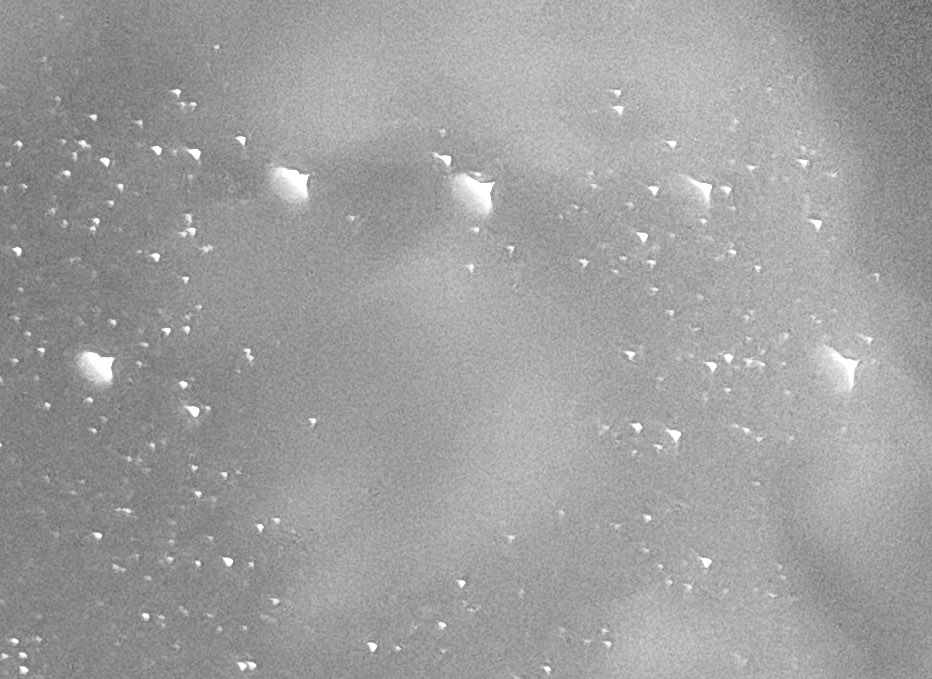
\includegraphics[width=0.4\tw]{img/optics-aberrations-coma.jpg}	
	\caption{Изображение <<хвоста>> Большой Медведицы, полученное с помощью широкоугольного объектива, страдающего ярко выраженной комой.}
	\label{pic:optics-aberrations-coma}
\end{wrapfigure}
Один из видов аберраций оптических систем~--- аберрация широкого пучка световых лучей, проходящий наклонно к оптической оси системы, как и \imp{сферическая аберрация}, обусловлена неодинаковым преломлением световых лучей различными участками линзовых компонент системы. Кома приводит к нарушению центрированности светового пучка. В результате такой аберрации изображение точки имеет вид несимметричного пятна (см.~Рис.\,\ref{pic:optics-aberrations-coma}), по форме напоминающего запятую (англ. {\itshape comma}).

































